\documentclass[tikz,border=10pt]{standalone}
\begin{document}
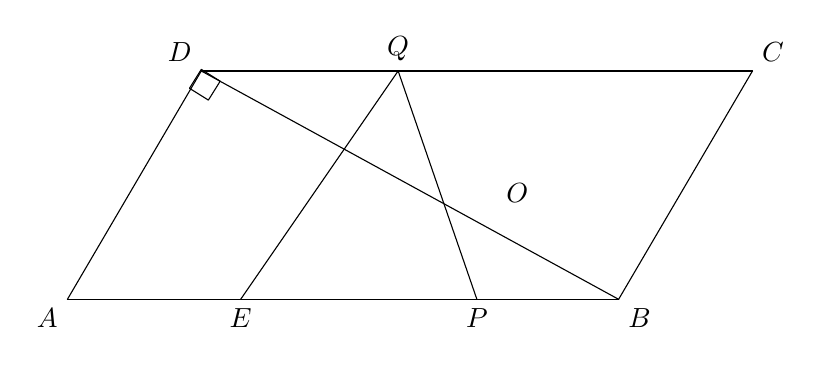
\begin{tikzpicture}[line cap=round,line join=round]

% Coordinates
\coordinate (A) at (0,0);
\coordinate (E) at (2.2,0);
\coordinate (P) at (5.2,0);
\coordinate (B) at (7.0,0);

\coordinate (D) at (1.7,2.9);
\coordinate (Q) at (4.2,2.9);
\coordinate (C) at (8.7,2.9);

% Intersection point for labeling
\coordinate (O) at (5.45,1.35);

% Outer boundary
\draw (A) -- (B);
\draw (A) -- (D);
\draw (D) -- (C);
\draw (B) -- (C);

% Inner segments
\draw (E) -- (Q);
\draw (Q) -- (P);
\draw (D) -- (B);

% Right-angle mark at D between DA and DB
\draw (1.55,2.68) -- (1.79,2.53) -- (1.94,2.77) -- (1.70,2.92) -- cycle;

% Labels
\node[below left] at (A) {$A$};
\node[below] at (E) {$E$};
\node[below] at (P) {$P$};
\node[below right] at (B) {$B$};

\node[above left] at (D) {$D$};
\node[above] at (Q) {$Q$};
\node[above right] at (C) {$C$};

\node[right] at (O) {$O$};

\end{tikzpicture}
\end{document}
